\chapter{Big Example}
\label{chap:big_example}
This chapter demonstrates how Distrace can be used on bigger example and also serves as the user manual for creating custom monitoring applications. We will show how all steps from creating the application up to running the application and seeing the observed results.

This example is based on the H\textsubscript{2}O\footnote{More information about H\textsubscript{2}O can be found on \url{https://www.h2o.ai} and \url{https://github.com/h2oai}} open-source fast scalable machine learning platform. This platform supports various methods for building machine learning models, methods such as deep learning, gradient boosting or random forests. The core of the tool is written in Java and clients for different languages exist as well. Internally, H\textsubscript{2}O is using map-reduce computation paradigm\footnote{Map-reduce is a programming model in distributed systems. The basic idea is to split tasks into smaller parts and perform the map operations. The intermediate results are then combined together using the reduce calls until the complete result has been assembled from all the sub-tasks.} to perform various tasks across the cluster.

The goal of this example is to monitor subset of map-reduce tasks and see visualization of the computation process. This can help reasoning about performance of the platform and can discover unwanted delays in computations. This chapter first describes relevant parts of the H2O platform in more details. Then in the following sections we describe in steps how to extend the core instrumentation library for H2O purposes. Lastly, we show how this example can be started and how visual output can be interpreted. 
This full example is also available in the attached source code of the thesis in the first attachment. More examples are available and the list and instructions on how they can be run is in the second attachment.

\section{H\textsubscript{2}O In More Details}
H\textsubscript{2}O is in-memory machine learning platform. The computations are performed in cluster, where the cluster consists of several H2O nodes. All nodes in the cluster are equal and each of them can initialize the computation. Each computation is performed as a map-reduce. This section first describes the format of data used in H2O and how data are stored and then how the computations is performed in the cluster. 

\subsection{Data in H\textsubscript{2}O}
Data are stored in H\textsubscript{2}O in so called \texttt{Frames}. Frame is an in-memory distributed data table with columns and rows. The \texttt{Frame} is designed in a way that it can handle data which are not possible to fit into a memory of a single machine. Each column is represented by the \texttt{Vec} class. This class represents vector of data that is again distributed across nodes in the cluster. Further, each vector is split into multiple \texttt{Chunk}s, where chunk is part of the vector actually stored on the single node. 

It is possible for one node to contain multiple chunks from a single frame and therefore, the number of chunks in a vector does not represent the number of nodes on which the data are distributed. Also, data imported to H\textsubscript{2}O are distributed via chunks equally among all the nodes in the cluster, but algorithm may also decide to distribute the data on just several nodes in the cluster. It is also possible to create the frame manually and specify on which nodes the chunks should be stored. Therefore, the frame may be distributed on only a portion of the cluster. Also, usually when chunks are being created on some specific node, chunks of the same size for each column are created on that node. This means that each node storing the data usually have corresponding chunks for all the columns. This can be though of that each node storing some data has a subset of rows from the full table with all columns.

The Figure \ref{fig:h2o_frame} shows the structure of frame with three columns, where each column is split into two chunks. It also shows how chunks may be distributed in the cluster of size three. It can also be seen that corresponding chunks for each vector have the same size and are stored on the same nodes. 

	\begin{figure}
		\centering
		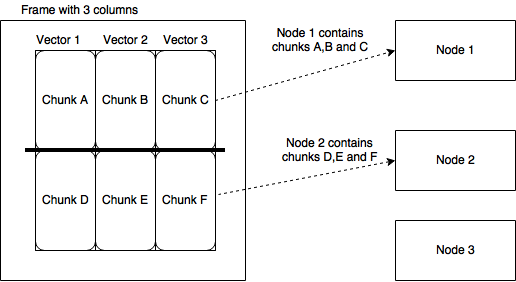
\includegraphics[scale=0.5]{h2o_frame.png}
		\caption{Structure of H\textsubscript{2}O frame and its distribution in the cluster.}
		\label{fig:h2o_frame}
	\end{figure}

\subsection{Computation in H\textsubscript{2}O}
For example, when the user tells H2O to create a deep learning model based in the data on the input, H2O sees this as a \textbf{Job}. Jobs are used to track long-lifetime user interactions and encapsulate the whole computation from the user point of view. The job can consist of several map-reduce tasks. In H2O, the class \texttt{MRTask} is used as the core implementation of the map-reduce tasks. The map-reduce task is always bound to some  H\textsubscript{2}O frames on which the computation needs to be performed. This class is used to encapsulate the task, partition it to a smaller tasks and run remote computations among the whole cluster. The \texttt{map} operations are called on the leaf tasks to compute the result based on the locally available data and \texttt{reduce} calls are used to reduce the result from two sub-tasks into a new task with combined result from the children.

In more detail, the class \texttt{MRTask} extends from \texttt{DTask}. This class is a general class used in H\textsubscript{2}O to represent task remote executed. Further, \texttt{DTask} extends from \texttt{H2OCountedCompleter}. The last class is a simple wrapper around the Fork/Join execution framework\footnote{For more information, please read Java documentation for Fork/Join framework available at \url{https://docs.oracle.com/javase/tutorial/essential/concurrency/forkjoin.html}.} allowing the platform to prioritize tasks. Fork/Join (F/J) framework is an implementation of Java \texttt{ExecutorService}, which helps with job parallelization on multiple processors. The Fork/Join thread framework execute tasks in separated threads and can move tasks between threads to ensure the highest possible performance. Each H\textsubscript{2}O \texttt{MRTask} is executed as \texttt{ForkJoinTask} inside this execution framework. A \texttt{ForkJoinTask} is a task wrapper which can run inside a single thread. It is a light-weight wrapper and big number of tasks may be served by a smaller number of actual threads.

The way how H\textsubscript{2}O perform computation from high-level point of view can be seen on the Figure \ref{fig:h2o_overview}. The task initiator receives the \texttt{MRTask} from the parent \texttt{Job} or from the user. It splits the task into two new sub-tasks and send these tasks to new nodes in the cluster. The intermediary nodes does the the splitting again and sends the task again to the another two selected nodes in the cluster. The leaf nodes does not split the task anymore.

	\begin{figure}
		\centering
		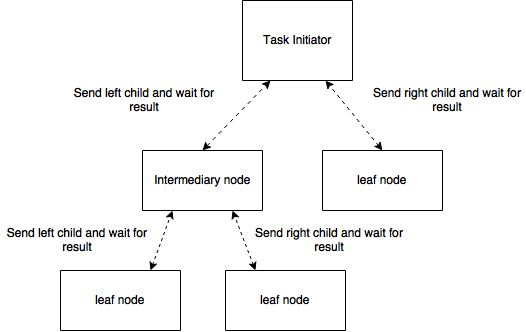
\includegraphics[scale=0.5]{h2o_overview.png}
		\caption{High-level overview of execution hierarchy.}
		\label{fig:h2o_overview}
	\end{figure}


It is important to say that the \texttt{MRTask} is always distributed to all nodes in the cluster. This figure shows how it is ensured that each node will be participating in the computation, however we still miss the computation step itself. Each node of the cluster who receives a task also submit this task for computation into the Fork/Join execution framework. This computation performs the mapping operation on all the chunks, which are available locally on the node executing this task, for the frame associated to the task. The \texttt{operation} follows the \texttt{map} operation, however we need to first ensure that the child tasks, from which we want to combine results together, are already finished. This is ensured by child tasks signaling the parent tasks when the work has been finished so parent tasks can know when they can start reducing the results.

The computation on the single node is shown in the following pseudo-code
\begin{lstlisting}[language=Java]
 MRTask task = ... // task received from the parent or from the user
 MRTask left = split(task, start1, end1)
 MRTask right = split(task, start2, end2)
 remoteCompute(left)
 remoteCompute(right)
 H2O.submitTask(task) // submit this task into F/J
..
// task is taken from F/J for execution
task.map(..)
task.waitForComplete() // wait for the child tasks to finish
task.reduce(left, right)

notifyComplete(task) // notify parent of completion
\end{lstlisting}
The split method accept also indices representing nodes in the cluster on which this sub-task and further sub-sub-tasks may be executed.

The last missing piece of information is what is done when the node has more chunks available for the frame associated with the task, since each \texttt{map} operation is executed only per single chunk. In case the node has multiple chunks available for the frame, the node always locally submits two new tasks into the F/J framework, each having half of the chunks. This is recursively repeated until we have tasks of size one chunk which are processed normally. These locally-split tasks signalize to their parents that they are done. This signalization goes up the tree until the original task is marked finished.

\subsection{Methods for Instrumentation}
For purpose of this example, a special \texttt{MRTask} called \texttt{SumMRTask} has been created. This task just perform distributed sum of the range of the numbers. In order to be able to visualize the computation process of this task, the following \texttt{MRtask} methods are important for the instrumentation
\begin{itemize}
	\item \texttt{dfork} - this method is called at the initiator node and starts the computation of the whole task.
	\item \texttt{getResult} - this method is also called at the initiator and blocks until the distributed computation finishes.
	\item \texttt{setupLocal0} - this method splits the task, creates sub-tasks for child nodes and finally submits the sub-tasks to the target child nodes.
	\item \texttt{map} - the map operation.
	\item \texttt{reduce2} - the reduce operation.
	\item \texttt{compute2} - this method handles the computation itself by calling the \texttt{map} implementation.
	\item \texttt{onComplete} - this method waits for the sub-tasks to finish and then calls \texttt{reduce2} on them.
\end{itemize}

We are also interested how long the remote computation lasted on child nodes. For this reason we need to instrument the following two methods on the \texttt{RPC} class:
\begin{itemize}
	\item \texttt{call} - this method is called when the remote computation has been submitted.
	\item \texttt{response} - this method is called when the remote computation has been finished and the child node is signaling that its work is done.
\end{itemize}

\section{Building the Core Server and Native Agent}
In order be able to extend the core instrumentation library, we need to build it first. This won't be necessary once the core instrumentation server is published to some online repository of JAR packages\footnote{For example, Maven Central Repository.} The native agent also needs to be built on the platfrom where H\textsubscript{2}O will be running. 

Please see the Attachment 3 for the information on how to build the project from sources or how to run this example from the prepared Docker machine. 

\section{Extending the Core Instrumentation Server}
In order to be able to capture the relationships between tasks and their computation, we need to instrument the method mentioned in the previous section. It is important to always find a good pair of methods which open and close a single span. In case of H\textsubscript{2}O the following calls have been identified to form a good spans. The pairs are ordered from the top level pairs encapsulation the whole computation up until the local spans encapsulation single mapping or reduce operations.

\begin{enumerate}
	\item \texttt{dfork} - \texttt{getResult}. This pair is used to open a main span which encapsulates the complete computation of a single \texttt{MRTask}, because \texttt{dfork} is only called on the node where the computation starts and the same holds for \texttt{getResult} on the same node after computation finished. The span is open when the first method is entered and closed when the later method is leaved.
		
	\item \texttt{setupLocal0} - \texttt{onCompletion}. This pair forms a span representing the complete communication on a single node. It encapsulates the local work as well as waiting for the remote work to complete in order to be able to call \texttt{reduce}. This span is opened when the first method is entered and leaved when the later method is leaved. This span is well-defined since for each task the \texttt{onCompletion} method is called and represents that the work has been finished at all children tasks.
	
	\item \texttt{call} - \texttt{response}. This pair forms a span used to track only remote computation. It encapsulates the remote computation and all following sub-tasks created by the remote task. This span is opened when the first method is entered and closed when the second method is leaved.
	
	\item \texttt{compute2} - \texttt{onCompletion}. This pair forms a span used to encapsulate computation on the local node. It encapsulates all the cases of local work. In case of multiple chunks exist for the given tasks on the same node, it is recursively called until we have tasks representing a single chunk. The calls are also recursively confirmed by the \texttt{onCompletion} call. In multi-chunk case, only one child task is submitted for execution into F/J thread. The second task is executed immediately in the same thread. This way it is ensured that we can reuse the existing threads as much as possible. This span is opened when the first method is entered and closed when the first method is leaved.
	
	\item \texttt{map} - \texttt{map}. This pair represents a single mapping operation. This span is entered when the \texttt{map} method is entered and closed when the \texttt{map} method is leaved. Therefore this span lasts only for duration of the \texttt{map} method call.
	
	\item \texttt{reduce2} - \texttt{reduce2}. This pair represents a single reduce operation. This span is entered when the \texttt{reduce2} method is entered and closed when the \texttt{reduce2} method is leaved. Therefore this span lasts only for duration of the \texttt{reduce 2} method call.
\end{enumerate}

For all of the pairs above, the Advice API is used for instrumentation because it's sufficient to be able to capture just method entered and method exit events. In case we would like to instrument more complex cases, we could use Interceptors API which is described in the Byte Buddy documentation and briefly also in the Section \ref{sec:byte_buddy}.

Instrumenting the methods is technical tasks and the code can be seen in the example. The trace context information is always attached to the tasks transferred. The trace context is initially created during the \texttt{dfork} method call, since it's the main entry point of the computation. When instrumenting \texttt{compute2} and \texttt{setupLocal0} methods, the deep copy of trace context is attached to the transferred task as the \texttt{onComplete} method is usually called from different thread and this ensures there are no collisions and multiple objects accessing the same trace context.

Also, when instrumenting a few of the mentioned methods we need to ensure that correct pairs of spans are created. For this purpose we use support for flags on the \texttt{Span} class. Flags allow us to attach additional information to trace context which may be used at the closing side of the span. This is for example useful in cases when a method is used to close several spans at the same time and we need to properly distinguish between the spans.

Once all the advices or onterceptors are created we need to create corresponding transformers which define the association between the method in the monitored application and the method used for the instrumentation. For this purpose, Distrace provides several helper methods allowing us to create transformers in a very concise way. For example, the transformer defining instrumentation of \texttt{call} and \texttt{response} method looks like:

\begin{lstlisting}[language=Java]
new BaseTransformer() {
@Override
public DynamicType.Builder<?> 	defineTransformation(
	DynamicType.Builder<?> builder) {

	Method call = ReflectionUtils.getMethod(RPC.class, "call");

	return builder.visit(Advice.to(RPCAdvices.call.class).on(is(call))).
	visit(Advice.to(RPCAdvices.response.class).on(named("response")));
}
});
\end{lstlisting}


Once all transformers are defined, we need to associate the transformers with the classes from the application on which they should operate and also create a main entry point of the extended instrumentation server we just created. This is demonstrated on the following code snippet:

\begin{lstlisting}[language=Java]
 public static void main(String args[]) {
	new Instrumentor().start(args, new MainAgentBuilder() {
		@Override
		public AgentBuilder createAgent(
			BaseAgentBuilder builder,
			String pathToHelperClasses) {
	 		 
			return builder.type(isSubTypeOf(MRTask.class))
			.transform(mrTaskTransformer)
			.type(is(RPC.class))
			.transform(rpcTransformer)
	         }
	  });
}			 
\end{lstlisting}
It can be seen in this code that we are starting the instrumentation server using the API provided by the core instrumentation server with the \texttt{MainAgentBuilder} instance. This instance is later used as a dispatcher of instrumentation of the whole application.

Later when starting the application with the attached native agent and configuring the agent, we need to explicitly specify the class, which is used as the main entry point. This is exactly the class containing the \texttt{main} method with the content above.

Now we need to build the extended instrumentation server. This server has two dependencies: the core instrumentation server and also the H\textsubscript{2}O application sources. The first dependency is obvious as we are using the API defined in the library. The second library is required since we used several application classes when defining the instrumentation points. This may not be necessary when instrumenting different applications since we can identify the class to be instrumented for example by its name as \texttt{named("fully.qualified.class.name)} instead of \texttt{is(Example.class)}. The second option however gives us more freedom when defining the instrumentation points and has also a performance benefit. In this case, the application classes are already located in the instrumentor and when they are requested to be instrumented, their original bytecode don't have to be sent from the native agent. 

After this step, we should have two artifacts - the native agent library built for our platform from the previous steps and also the extended instrumentation server JAR file from this step.
\section{Configuring and Running the Application}
For the purposes of this example, we will start a cluster of three H\textsubscript{2}O nodes. Two nodes will be the regular nodes and the last node will contain the main method in which we execute the the \textbf{SumMRTask}. This task is used to sum range of the numbers in distributed manner.

Arbitrary H\textsubscript{2}O node can be started as: \newline \texttt{java -jar h2o.jar -name cluster\_name}\newline When operating on the network with multi-cast communication enabled multiple nodes started with the same cluster name will form a cluster.

If we want to start the application with the monitoring agent attached, we can use the \texttt{-agentlib} java option. Any H\textsubscript{2}O node can be started with the monitoring feature enabled just by calling the following command: \newline
\texttt{java -agentpath:"\$NATIVE\_AGENT\_LIB\_PATH=\$AGENT\_ARGS" -jar h2o.jar  \newline -name cluster\_name}

The \texttt{\$NATIVE\_AGENT\_LIB\_PATH} needs to point to the location of the native agent library and \texttt{\$AGENT\_ARGS} shell variable may contain any arguments passed to the native agent. The arguments are in the format \texttt{key=value} and are separated by the semicolon.

In case of this example, we will let the native agent to start the instrumentation server locally for each node automatically. Therefore, the inter-process communication will be used and we don't need to configure it explicitly. Only two arguments need to be specified - the path to the instrumentation server and the fully qualified name of the main entry class.

Therefore, the full command starting H\textsubscript{2}O with the monitoring agent enabled can be : \newline
\texttt{java -agentpath:"/home/agent.so=instrumentor\_server\_jar=\newline/home/instrumentor.jar;instrumentor\_main\_class=main.entry.pint" \newline-jar h2o.jar -name cluster\_name}

In order to start the cluster of size three, we need to call this command three times, two times with the regular H\textsubscript{2}O node and once with the H\textsubscript{2}O node containing the execution of the \texttt{SumMRTask}. It is also important to start the Zipkin user interface to which the results are published. The user interface server may be started as: \texttt{java -jar zipkin.jar}\footnote{Zipkin Jar file may be downloaded at \url{https://github.com/openzipkin/zipkin} or is available at the attached CD.}.
\section{The Results}
Once all three nodes have been started, the computation starts and the results based on our instrumentation will be shown directly in the Zipkin user interface. By default, the user interface is available at port 9411.

We need to click on the \textit{Find Traces} button to show all traces, which satisfy the search conditions. We should see in the output a single trace and once we click on it, we should see similar result to the one on the Figure \ref{h2o_zipkin_output}. This figure shows just portion of the whole trace, but contains the important observed information.
	\begin{figure}
		\centering
		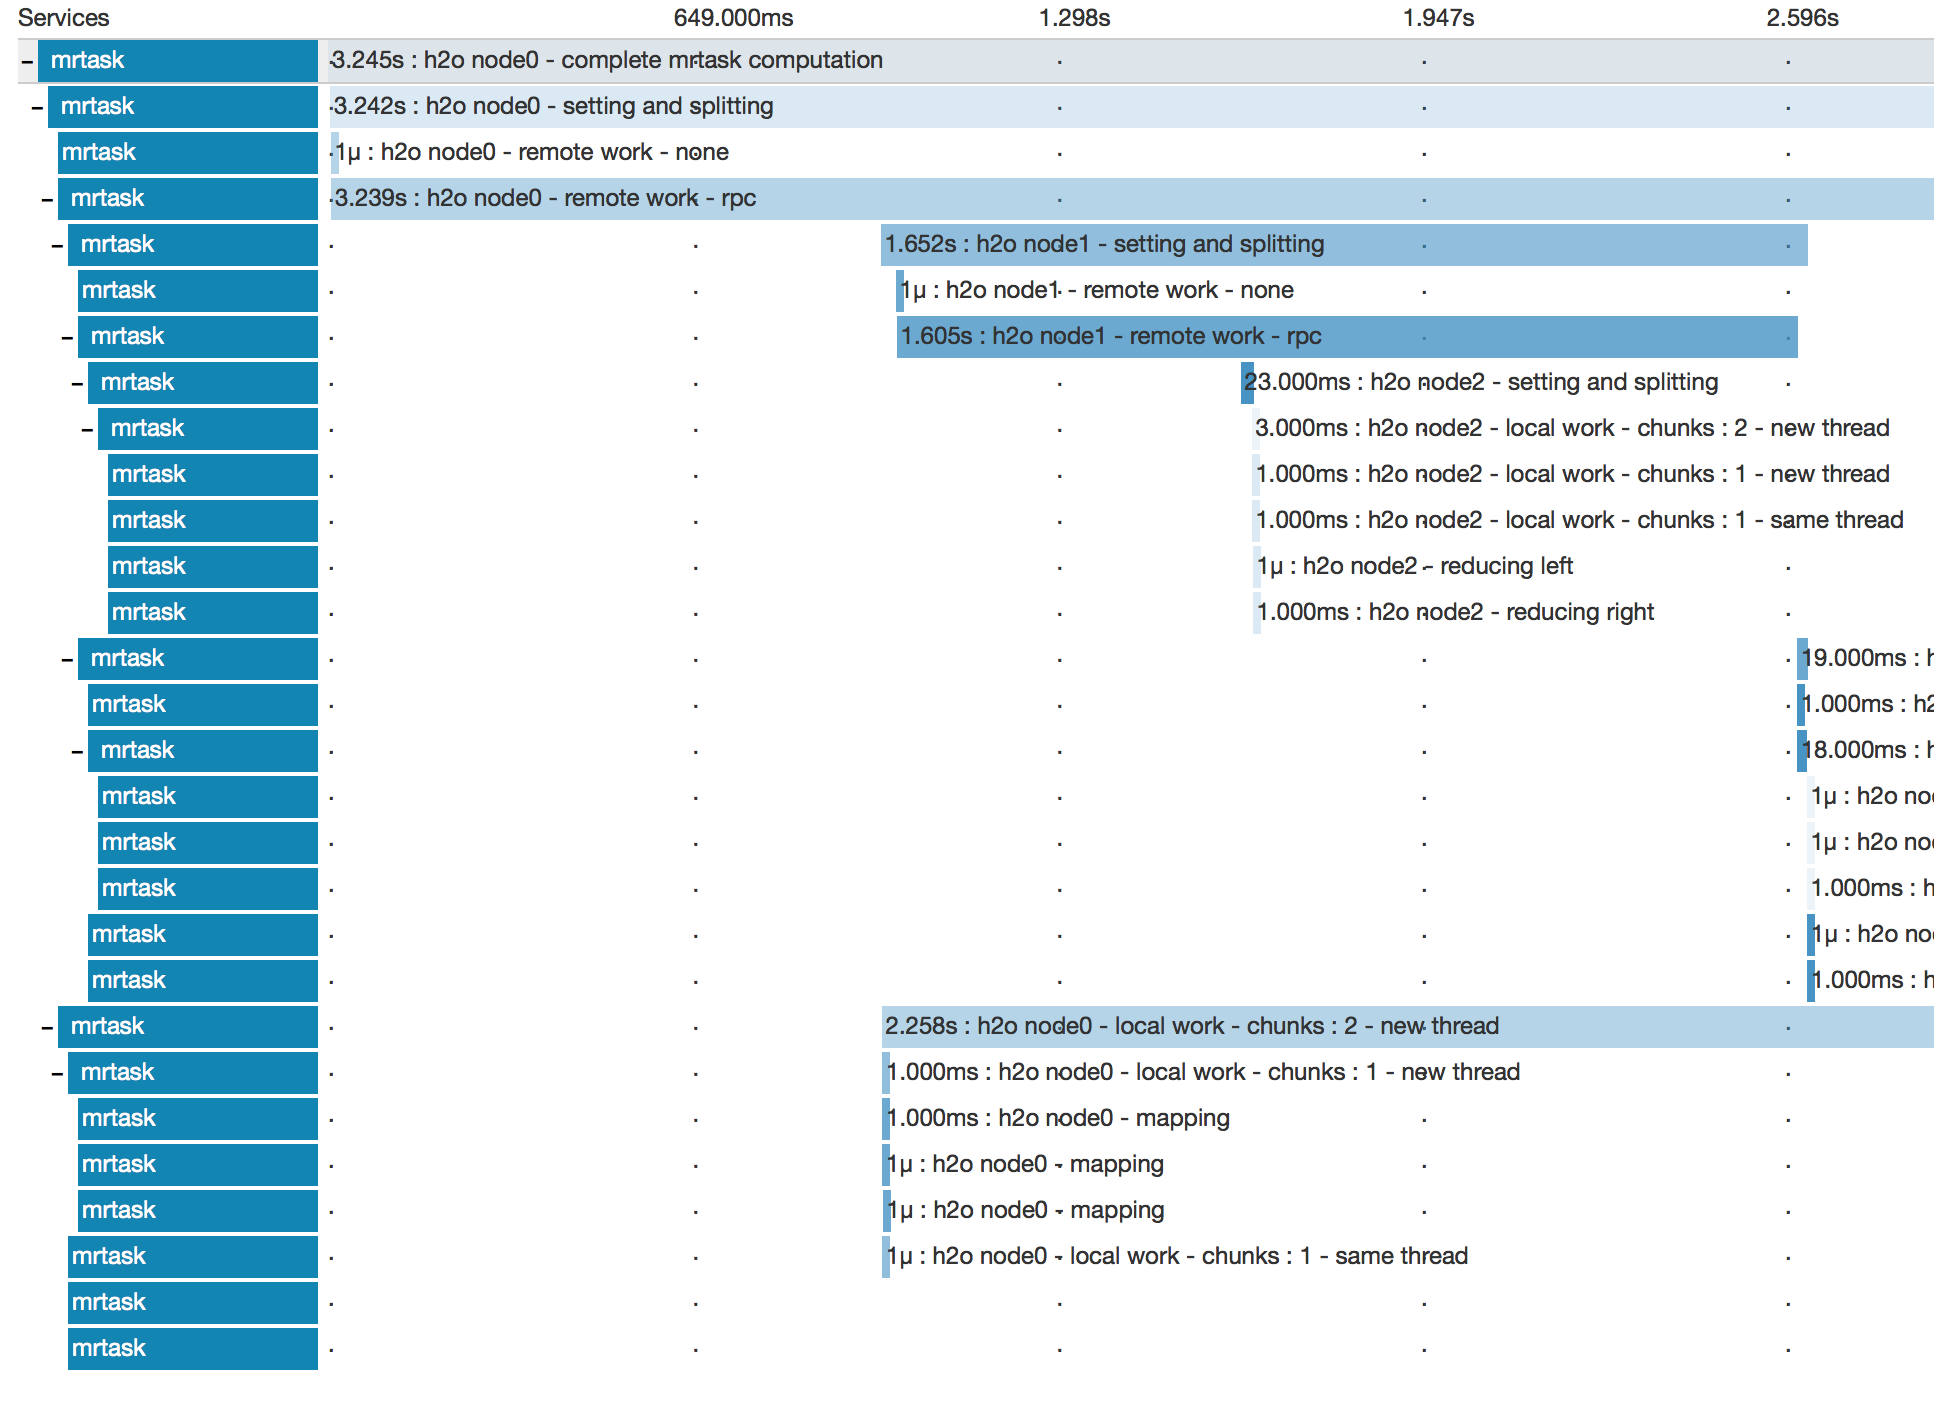
\includegraphics[scale=0.4]{h2o_zipkin_output.png}
		\caption{Example trace from the distributed computation on H\textsubscript{2}O}
		\label{h2o_zipkin_output}
	\end{figure}

All the operations and their timing can be seen on the output and we can see how long each operation lasted and when it started. The spans are also organized hierarchically as they were created. We can see the main span encapsulating the whole computation, the spans for computation on each node and also spans encapsulation the remote computations. The local \texttt{map} and \texttt{reduce} calls are displayed as well. It is, for example, interesting to see how long it took the platform to perform the \texttt{reduce} operation after the \texttt{map} operation has been called.